% !TEX root =  ../00_thesis.tex

% ------------------------------------------------------------------------------
% Global Positioning
In the previous chapter, we discussed how to design and analyze networking experiments in general~(\cref{ch:triscale}).
In the rest of this dissertation, we will focus on low-power wireless networking, and more specifically on a technique called \emph{synchronous transmissions}.

% ------------------------------------------------------------------------------
% Context
Synchronous transmissions (\ST) refers to a wireless approach for broadcasting messages in a multi-hop network using flooding.
This is made efficient by letting multiple transmitters send the \emph{same packet} at the \emph{same time}; hence the name of \emph{synchronous} transmissions.%
\footnote{The name \textsl{concurrent transmissions} is also found in the literature.}
\ST has been proven highly reliable and energy efficient for low-power wireless networks.
Furthermore, \ST supports mobility by design thanks to the stateless logic of flooding-based communication.

% ------------------------------------------------------------------------------
% What is the problem?
Unfortunately, it is difficult to guarantee that multiple nodes actually send at the ``same time''.
The required precision on synchronization depends, \eg on the physical layer speed, the radio modulation speed or the encoding scheme.
For typical low-power wireless motes available today, the synchronization must be in the order of \us for \ST to work reliably.
Achieving such time synchronization requires to precisely control the timing of radio operations, which involves careful timer settings and interrupt handling.
The integration of such ``low-level software'' within a entire network stack is challenging.
Consequently, the adoption and development of \ST-based network stacks has been hindered by
the lack of usable and flexible design tools.

\begin{figure}
  \centering
  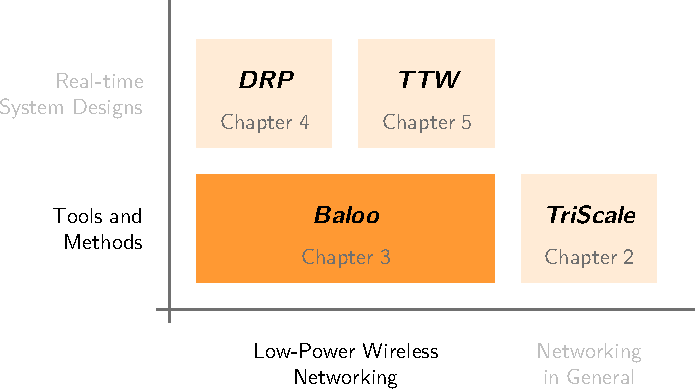
\includegraphics[scale=0.9]{chapter_baloo}
  \caption{Positioning of this chapter in the dissertation.
  \capt{This chapter presents \baloo, a design framework facilitating the implementation of low-power wireless networking protocols based on synchronous transmissions.}}
  \label{fig:chapter_baloo}
\end{figure}

% ------------------------------------------------------------------------------
% Claim
Thus, in this chapter, we study the feasibility of a design tool that would facilitate the development of network stacks based on \ST~(\cref{fig:chapter_baloo}); typically, such a tool would be useful for implementing our real-time protocol stacks (see \cref{ch:drp} and \cref{ch:ttw}).

\fakepar{Claim}
We propose and implement \baloo, a design framework for network stacks based on synchronous transmissions.
\baloo significantly lowers the entry barrier for harnessing the efficiency, reliability and mobility support of synchronous transmissions: users implement their protocol through a simple yet flexible API while \baloo handles all the complex low-level operations based on the users' inputs.

\baloo is flexible enough to implement a wide variety of network layer protocols, with only limited memory and energy overhead.

% ------------------------------------------------------------------------------
% Corresponding reference(s)
\begin{publi}

  The material from this chapter builds upon the work from Jonas Bächli~\cite{bachli2018Creating}. It relates to the following publication.

  \inlineRef{Synchronous Transmissions Made Easy: Design Your Network Stack with Baloo}{Romain Jacob, Jonas Bächli, Reto Da Forno, Lothar Thiele}{EWSN 2019. Beijung, China (February 2019)}

\end{publi}

% ------------------------------------------------------------------------------
% ------------------------------------------------------------------------------
% FORMER INTRO
% ------------------------------------------------------------------------------
% ------------------------------------------------------------------------------
% \newpage
% %Context
% \textsl{Synchronous Transmissions} (\ST) refers to a wireless communication technique that broadcast messages in a multi-hop network using flooding.
% This is made efficient by letting multiple transmitters send the \textsl{same packet} at the \textsl{same time}; henceforth the name of \emph{synchronous} transmissions.%
% \footnote{The name \textsl{concurrent transmissions} is also found in the literature.}
% \ST has been proven to be highly reliable and energy efficient, in particular for low-power wireless networks. Furthermore, flooding allows \ST to seamlessly support mobility by design.
% More informantion about \ST are presented in Introduction (\cref{ch:introduction}).
%
% %Problem
% Unfortunately, it is difficult to guarantee that multiple nodes actually send at the ``same time''.
% The required precision on synchronization depends \eg on the physical layer speed, the radio modulation speed or the encoding scheme.
% For typical low-power wireless motes available today, the synchronization must be in the order of \us for \ST to work reliably.
% Achieving such time synchronization requires to precisely control the timing of radio operations, which involves careful timer settings and interrupt handling.
% The integration of such ``low-level software'' within a entire network stack is challenging.
% Consequently, the adoption and development of \ST-based network stacks has been hindered by
% the lack of usable and flexible design tools.
%
% %Task and object
% Therefore, we developed \baloo: a flexible network stack design framework, designed to facilitate the development of protocols based on \ST. The key element of \baloo is a middleware layer which separates the radio management from the protocol implementation: \baloo provides a flexible application programming interface, while ensuring the correct timing of radio operations.
%
% %Findings
% \baloo is flexible enough to implement a wide variety of network layer protocols, with only limited memory and energy overhead.
% Most importantly \baloo makes \ST accessible: The software is open source and well documented.
% Since its development, \baloo has been used in a variety of projects, from both our team and external research groups.
% We believe that \baloo is an important enabler for a whole new class of Internet of Things applications leveraging the reliability, efficiency, and flexibility of \ST.

%
%
% This chapter presents \baloo, its design and the evaluation of its performance. We conclude with a brief description of projects that have been facilitated by \baloo, and finally discuss potential future developments, including standardization efforts.
